% ============================================================================
% Section 5: Transaction Format
% ============================================================================

\section{Transaction Format}
\label{sec:transactions}

\subsection{Transaction Types}

\Botho supports two transaction types:

\begin{table}[h]
\centering
\caption{Transaction type comparison}
\label{tab:tx-types}
\begin{tabular}{@{}lccccl@{}}
\toprule
\textbf{Type} & \textbf{Inputs} & \textbf{Outputs} & \textbf{Signature} & \textbf{Size} & \textbf{Use Case} \\
\midrule
Minting & 0 & 1--16 & ML-DSA-65 & $\sim$2 KB & Block rewards \\
Private & 1--16 & 1--16 & CLSAG & $\sim$4 KB & All transfers \\
\bottomrule
\end{tabular}
\end{table}

\subsection{Private Transaction Structure}

A private transaction transfers value while hiding sender, recipient,
and amount.

% Transaction Anatomy Diagram
% Visual breakdown of all transaction components with size annotations
%
% ACCESSIBILITY ALT TEXT:
% A structural diagram showing the components of a Botho transaction. The
% main box contains: Header (32 bytes) at top, Inputs section (each 680
% bytes with ring references and key image), Outputs section (each 1152
% bytes with commitment, stealth key, and KEM ciphertext), CLSAG signatures
% (704 bytes per input), and Bulletproof range proof (736 bytes aggregated).
% Total transaction size is approximately 4.5 KB for a typical 1-input,
% 2-output transaction.

\begin{figure}[ht]
\centering
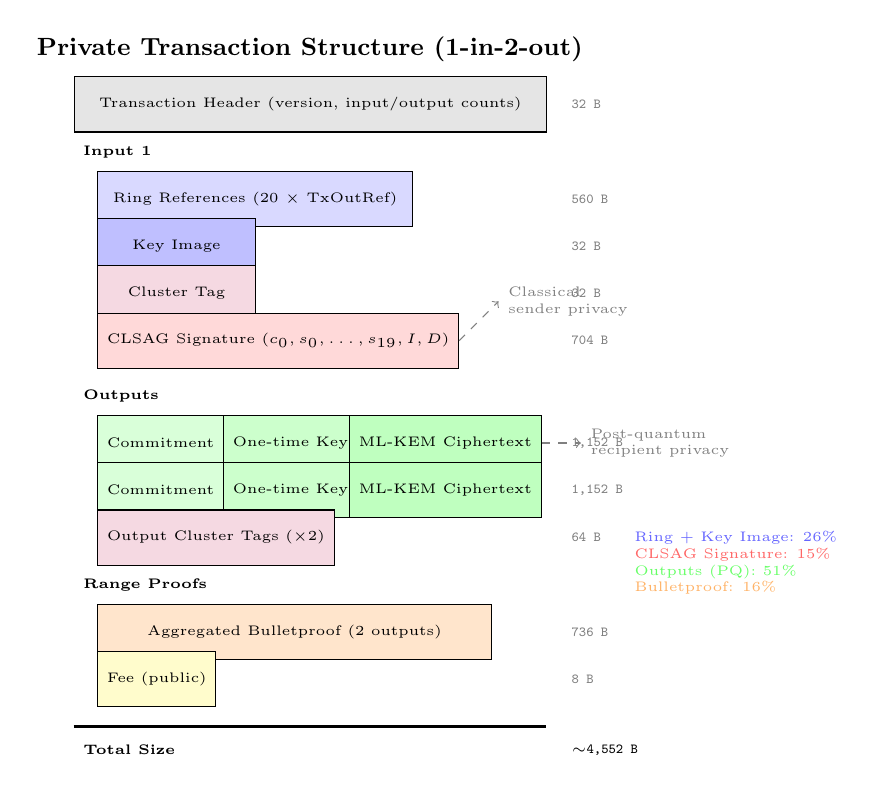
\begin{tikzpicture}[
    component/.style={draw, rectangle, minimum height=0.7cm, font=\tiny, anchor=west},
    label/.style={font=\tiny, anchor=east},
    size/.style={font=\tiny\ttfamily, anchor=west, text=gray}
]
    % Title
    \node[font=\small\bfseries] at (3,5.5) {Private Transaction Structure (1-in-2-out)};

    % Header section
    \node[component, fill=gray!20, minimum width=6cm] (header) at (0,4.8) {Transaction Header (version, input/output counts)};
    \node[size] at (6.2,4.8) {32 B};

    % Input section header
    \node[font=\tiny\bfseries, anchor=west] at (0,4.2) {Input 1};

    % Ring references
    \node[component, fill=blue!15, minimum width=4cm] (ring) at (0.3,3.6) {Ring References (20 $\times$ TxOutRef)};
    \node[size] at (6.2,3.6) {560 B};

    % Key image
    \node[component, fill=blue!25, minimum width=2cm] (keyimg) at (0.3,3.0) {Key Image};
    \node[size] at (6.2,3.0) {32 B};

    % Cluster tag (input)
    \node[component, fill=purple!15, minimum width=2cm] (intag) at (0.3,2.4) {Cluster Tag};
    \node[size] at (6.2,2.4) {32 B};

    % CLSAG signature
    \node[component, fill=red!15, minimum width=4.5cm] (clsag) at (0.3,1.8) {CLSAG Signature ($c_0, s_0, \ldots, s_{19}, I, D$)};
    \node[size] at (6.2,1.8) {704 B};

    % Output section header
    \node[font=\tiny\bfseries, anchor=west] at (0,1.1) {Outputs};

    % Output 1
    \node[component, fill=green!15, minimum width=1.5cm] (out1com) at (0.3,0.5) {Commitment};
    \node[component, fill=green!20, minimum width=1.5cm] (out1key) at (1.9,0.5) {One-time Key};
    \node[component, fill=green!25, minimum width=2cm] (out1kem) at (3.5,0.5) {ML-KEM Ciphertext};
    \node[size] at (6.2,0.5) {1,152 B};

    % Output 2
    \node[component, fill=green!15, minimum width=1.5cm] (out2com) at (0.3,-0.1) {Commitment};
    \node[component, fill=green!20, minimum width=1.5cm] (out2key) at (1.9,-0.1) {One-time Key};
    \node[component, fill=green!25, minimum width=2cm] (out2kem) at (3.5,-0.1) {ML-KEM Ciphertext};
    \node[size] at (6.2,-0.1) {1,152 B};

    % Output cluster tags
    \node[component, fill=purple!15, minimum width=3cm] (outtags) at (0.3,-0.7) {Output Cluster Tags ($\times$2)};
    \node[size] at (6.2,-0.7) {64 B};

    % Bulletproof section
    \node[font=\tiny\bfseries, anchor=west] at (0,-1.3) {Range Proofs};

    \node[component, fill=orange!20, minimum width=5cm] (bp) at (0.3,-1.9) {Aggregated Bulletproof (2 outputs)};
    \node[size] at (6.2,-1.9) {736 B};

    % Fee
    \node[component, fill=yellow!20, minimum width=1.5cm] (fee) at (0.3,-2.5) {Fee (public)};
    \node[size] at (6.2,-2.5) {8 B};

    % Total bar
    \draw[thick] (0,-3.1) -- (6,-3.1);
    \node[font=\tiny\bfseries, anchor=west] at (0,-3.4) {Total Size};
    \node[font=\tiny\ttfamily\bfseries, anchor=west] at (6.2,-3.4) {$\sim$4,552 B};

    % Size breakdown pie-style annotation
    \node[font=\tiny, align=left, anchor=north west] at (7,-0.5) {
        \textcolor{blue!60}{Ring + Key Image: 26\%}\\
        \textcolor{red!60}{CLSAG Signature: 15\%}\\
        \textcolor{green!60}{Outputs (PQ): 51\%}\\
        \textcolor{orange!60}{Bulletproof: 16\%}
    };

    % Annotation arrows
    \draw[->, gray, dashed] (out1kem.east) -- ++(0.5,0) node[right, font=\tiny, align=left] {Post-quantum\\recipient privacy};

    \draw[->, gray, dashed] (clsag.east) -- ++(0.5,0.5) node[right, font=\tiny, align=left] {Classical\\sender privacy};

\end{tikzpicture}
\caption{Anatomy of a private transaction (1 input, 2 outputs). The ML-KEM
ciphertext dominates output size (1,088 bytes each) but provides post-quantum
recipient privacy. Ring signatures use classical CLSAG for efficiency. Total
size is approximately 4.5 KB, compared to $\sim$50 KB with post-quantum ring
signatures.}
\label{fig:tx-anatomy}
\end{figure}


\subsubsection{Transaction Components}

\begin{lstlisting}[language=,caption={Private transaction structure}]
PrivateTransaction {
    prefix: TransactionPrefix,
    ring_signatures: Vec<CLSAGSignature>,
    bulletproofs: AggregatedRangeProof,
}

TransactionPrefix {
    version: u8,
    inputs: Vec<TxInput>,
    outputs: Vec<TxOutput>,
    fee: u64,
    extra: Vec<u8>,
}
\end{lstlisting}

\subsubsection{Input Structure}

Each input references a previously unspent output without revealing which:

\begin{lstlisting}[language=,caption={Transaction input structure}]
TxInput {
    ring: [TxOutRef; RING_SIZE],  // RING_SIZE = 20
    key_image: KeyImage,           // 32 bytes
    cluster_tag: ClusterTag,       // 32 bytes
}

TxOutRef {
    block_height: u64,
    tx_index: u16,
    output_index: u8,
}
\end{lstlisting}

The \texttt{ring} contains references to 20 possible source outputs.
The \texttt{key\_image} uniquely identifies the spent output (for
double-spend prevention) without revealing which ring member it
corresponds to.

\subsubsection{Output Structure}

Each output contains the encrypted amount and one-time keys:

\begin{lstlisting}[language=,caption={Transaction output structure}]
TxOutput {
    commitment: CompressedPoint,      // Pedersen commitment (32 bytes)
    one_time_key: CompressedPoint,    // One-time public key (32 bytes)
    encrypted_amount: [u8; 32],       // AES-encrypted amount
    ml_kem_ciphertext: [u8; 1088],    // ML-KEM ciphertext
    cluster_tag: ClusterTag,          // Derived from input tags
}
\end{lstlisting}

\subsection{Minting Transaction Structure}

Minting transactions create new coins as block rewards:

\begin{lstlisting}[language=,caption={Minting transaction structure}]
MintingTransaction {
    block_height: u64,
    nonce: u64,
    minter_public_key: MLDSAPublicKey,  // 1,952 bytes
    outputs: Vec<TxOutput>,
    signature: MLDSASignature,           // 3,309 bytes
}
\end{lstlisting}

Unlike private transactions:
\begin{itemize}
  \item No inputs (new coins created)
  \item Public amounts (for supply auditability)
  \item Known sender (minter identity is public)
  \item Recipients still hidden via stealth addresses
\end{itemize}

\subsection{Cluster Tags and Progressive Fees}
\label{sec:cluster-tags}

Cluster tags enable Sybil-resistant progressive fees by tracking coin
\textit{provenance} rather than current ownership. The key insight is that
splitting coins does not change where they came from.

% Cluster Tag Inheritance Diagram
% Shows tag blending when combining inputs from different clusters
%
% ACCESSIBILITY ALT TEXT:
% A flow diagram showing how cluster tags blend when combining inputs.
% Two input UTXOs are shown: one with 70% Cluster A tag (10 BTH) and one
% with 30% Cluster B tag (5 BTH). Arrows flow into a transaction box.
% The output shows a blended tag vector: the new UTXO has proportional
% attribution (70% A, 30% B based on input values). This tracking enables
% progressive fees based on coin ancestry without revealing ownership.

\begin{figure}[ht]
\centering
\begin{tikzpicture}[
    utxo/.style={draw, rectangle, rounded corners, minimum width=2.2cm, minimum height=1.2cm, font=\scriptsize},
    tag/.style={font=\tiny, fill=white, inner sep=1pt},
    arrow/.style={->, >=stealth, thick}
]
    % Title
    \node[font=\small\bfseries] at (0,4) {Cluster Tag Inheritance via Value-Weighted Blending};

    % Input UTXOs
    \node[utxo, fill=blue!20] (utxo1) at (-3.5,2) {
        \begin{tabular}{c}
            \textbf{UTXO 1}\\
            70 BTH
        \end{tabular}
    };
    \node[tag, below=0.1cm of utxo1] {Tag: $\{(A, 1.0)\}$};

    \node[utxo, fill=red!20] (utxo2) at (-3.5,0) {
        \begin{tabular}{c}
            \textbf{UTXO 2}\\
            30 BTH
        \end{tabular}
    };
    \node[tag, below=0.1cm of utxo2] {Tag: $\{(B, 1.0)\}$};

    % Transaction box
    \node[draw, rectangle, fill=gray!10, minimum width=1.5cm, minimum height=2.5cm, font=\scriptsize] (tx) at (0,1) {
        \begin{tabular}{c}
            \\
            \textbf{TX}\\
            \\
        \end{tabular}
    };

    % Blending formula inside TX
    \node[font=\tiny, align=center] at (0,1) {
        blend\\
        $\frac{\sum v_i \vec{t}_i}{\sum v_i}$
    };

    % Output UTXOs
    \node[utxo, fill=purple!20] (out1) at (3.5,2) {
        \begin{tabular}{c}
            \textbf{Output 1}\\
            60 BTH
        \end{tabular}
    };
    \node[tag, below=0.1cm of out1] {Tag: $\{(A, 0.7), (B, 0.3)\}$};

    \node[utxo, fill=purple!20] (out2) at (3.5,0) {
        \begin{tabular}{c}
            \textbf{Output 2}\\
            40 BTH
        \end{tabular}
    };
    \node[tag, below=0.1cm of out2] {Tag: $\{(A, 0.7), (B, 0.3)\}$};

    % Arrows
    \draw[arrow, blue!60] (utxo1.east) -- (tx.west |- utxo1.east);
    \draw[arrow, red!60] (utxo2.east) -- (tx.west |- utxo2.east);
    \draw[arrow, purple!60] (tx.east |- out1.west) -- (out1.west);
    \draw[arrow, purple!60] (tx.east |- out2.west) -- (out2.west);

    % Fee annotation
    \node[font=\tiny, gray] at (0,-0.8) {(fee not shown)};

    % Calculation box
    \node[draw, rectangle, rounded corners, fill=yellow!10, minimum width=7cm, font=\tiny, align=left] at (0,-2) {
        \textbf{Blending Calculation:}\\[2pt]
        $\vec{t}_{out} = \frac{70 \cdot \{(A,1.0)\} + 30 \cdot \{(B,1.0)\}}{70 + 30} = \{(A, 0.7), (B, 0.3)\}$\\[2pt]
        All outputs inherit the same blended tag regardless of their individual amounts.
    };

    % Key insight
    \node[draw, rectangle, rounded corners, fill=green!10, minimum width=7cm, font=\tiny, align=center] at (0,-3.5) {
        \textbf{Sybil Resistance:} Splitting coins does not reduce cluster attribution.\\
        A 100 BTH UTXO split into 100 $\times$ 1 BTH UTXOs all carry the same tag.
    };

    % Visual tag representation
    \node[font=\tiny\bfseries] at (-3.5,-4.5) {Input Tags};
    \draw[fill=blue!40] (-4.5,-5) rectangle (-2.5,-5.3);
    \node[font=\tiny, white] at (-3.5,-5.15) {100\% Cluster A};

    \draw[fill=red!40] (-4.5,-5.5) rectangle (-2.5,-5.8);
    \node[font=\tiny, white] at (-3.5,-5.65) {100\% Cluster B};

    \node[font=\tiny\bfseries] at (3.5,-4.5) {Output Tag};
    \draw[fill=blue!40] (2.1,-5) rectangle (3.5,-5.3);
    \draw[fill=red!40] (3.5,-5) rectangle (4.9,-5.3);
    \node[font=\tiny, white] at (2.8,-5.15) {70\% A};
    \node[font=\tiny, white] at (4.2,-5.15) {30\% B};

\end{tikzpicture}
\caption{Cluster tag inheritance through value-weighted blending. When a
transaction combines inputs from different clusters, the output tag vector
is the value-weighted average of input tags. This preserves provenance
information and ensures that splitting coins cannot reduce the cluster factor
used for progressive fee calculation.}
\label{fig:cluster-inheritance}
\end{figure}


\subsubsection{Tag Vector Representation}

Each UTXO carries a \textit{tag vector} representing the weighted distribution
of its ancestry across all clusters:

\begin{equation}
\vec{t} = \{(c_1, w_1), (c_2, w_2), \ldots, (c_k, w_k)\} \quad \text{where} \sum_i w_i = 1
\end{equation}

Here $c_i$ is a cluster identifier and $w_i$ is the fraction of the UTXO's
value attributable to that cluster.

\subsubsection{Cluster Creation at Minting}

Each minting transaction creates a new cluster. The minter's public key
hash serves as the cluster identifier:

\begin{equation}
c_{\text{new}} = \Hash(\text{minter\_pubkey} \| \text{block\_height})
\end{equation}

Minting outputs carry a tag vector with 100\% attribution to the new cluster:
$\vec{t}_{\text{mint}} = \{(c_{\text{new}}, 1.0)\}$.

\subsubsection{Tag Inheritance and Blending}

When spending multiple inputs, output tags are computed via value-weighted
blending:

\begin{equation}
\vec{t}_{\text{out}} = \frac{\sum_i v_i \cdot \vec{t}_i}{\sum_i v_i}
\end{equation}

where $v_i$ is the value of input $i$ and $\vec{t}_i$ is its tag vector.

\textbf{Example}: Combining a 70 BTH UTXO (100\% cluster A) with a 30 BTH
UTXO (100\% cluster B) produces output tags: $\{(A, 0.7), (B, 0.3)\}$.

\subsubsection{Age-Based Tag Decay}

To encourage circulation and prevent wash trading, tags decay over time.
However, decay only applies when UTXOs meet an age threshold:

\begin{equation}
\vec{t}'_i = \begin{cases}
0.95 \cdot \vec{t}_i & \text{if age}(\text{UTXO}_i) \geq T_{\min} \\
\vec{t}_i & \text{otherwise}
\end{cases}
\end{equation}

where $T_{\min} = 720$ blocks ($\approx$ 2 hours at 10s blocks).

\textbf{Wash Trading Resistance}: Since new outputs must wait before decay
applies, rapid self-transfers achieve no decay:

\begin{table}[h]
\centering
\caption{Tag decay limits}
\label{tab:decay-limits}
\begin{tabular}{@{}lcc@{}}
\toprule
\textbf{Attack} & \textbf{Transactions} & \textbf{Maximum Decay} \\
\midrule
Rapid wash (1 minute) & 100 & 0\% \\
Patient wash (1 day) & 1000 & 46\% \\
Patient wash (1 week) & 7000 & 97\% \\
\bottomrule
\end{tabular}
\end{table}

\subsubsection{Cluster Factor Calculation}

The cluster factor is derived from the dominant cluster's total minted wealth:

\begin{equation}
\text{cluster\_factor} = 1 + 5 \cdot \sigma\left(\frac{W_{\max}}{\text{steepness}}\right)
\end{equation}

where $W_{\max}$ is the total BTH ever minted by the dominant cluster and
$\sigma(x) = x/(1+x)$ is a sigmoid function.

\begin{table}[h]
\centering
\caption{Progressive fee multipliers}
\label{tab:fee-multipliers}
\begin{tabular}{@{}lc@{}}
\toprule
\textbf{Cluster Wealth Percentile} & \textbf{Fee Multiplier} \\
\midrule
Bottom 50\% & 1.0$\times$ -- 1.5$\times$ \\
50th -- 90th & 1.5$\times$ -- 3.0$\times$ \\
Top 10\% & 3.0$\times$ -- 6.0$\times$ \\
\bottomrule
\end{tabular}
\end{table}

% Progressive Fee Curve Diagram
% Shows fee multiplier as a function of cluster wealth percentile
%
% ACCESSIBILITY ALT TEXT:
% A line graph showing progressive fee structure. X-axis shows wealth
% percentile (0-100%), Y-axis shows fee multiplier (1x-6x). The curve is
% flat at 1x for bottom 50%, rises gently to 1.5x at 70%, steeper to 3x at
% 90%, then sharply to 6x for top 1%. Shaded regions show increasing fee
% intensity. Vertical dashed lines mark 50%, 90%, and 99% thresholds. The
% design ensures typical users pay base fees while wealth concentration
% faces economic pressure through higher transaction costs.

\begin{figure}[ht]
\centering
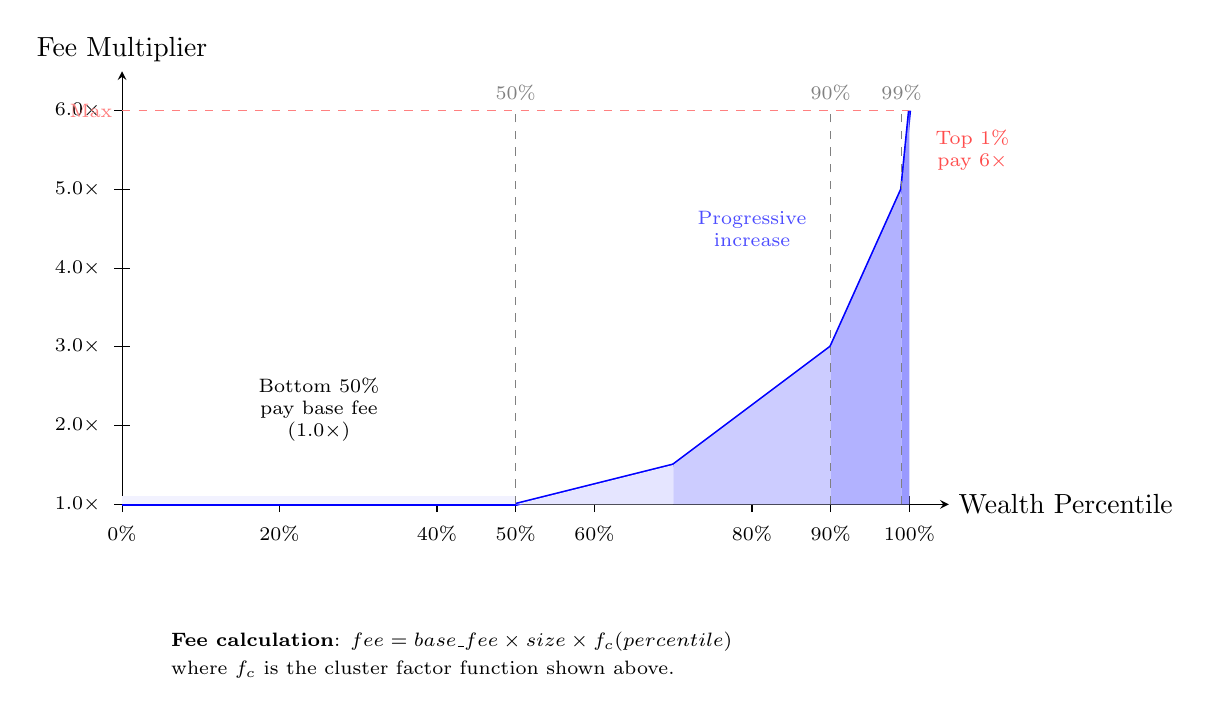
\begin{tikzpicture}[
    scale=1,
    >=stealth,
]

% Axes
\draw[->] (0,0) -- (10.5,0) node[right] {Wealth Percentile};
\draw[->] (0,0) -- (0,5.5) node[above] {Fee Multiplier};

% Y-axis labels
\foreach \y/\label in {0/1.0$\times$, 1/2.0$\times$, 2/3.0$\times$, 3/4.0$\times$, 4/5.0$\times$, 5/6.0$\times$} {
    \draw (-0.1,\y) -- (0.1,\y);
    \node[left] at (-0.15,\y) {\scriptsize \label};
}

% X-axis labels
\foreach \x/\label in {0/0\%, 2/20\%, 4/40\%, 5/50\%, 6/60\%, 8/80\%, 9/90\%, 10/100\%} {
    \draw (\x,-0.1) -- (\x,0.1);
    \node[below] at (\x,-0.15) {\scriptsize \label};
}

% Progressive fee curve (piecewise linear approximation of sigmoid-like curve)
% Bottom 50%: flat at 1x
\draw[very thick, blue] (0,0) -- (5,0);
% 50-70%: gentle rise to 1.5x
\draw[very thick, blue] (5,0) -- (7,0.5);
% 70-90%: steeper rise to 3x
\draw[very thick, blue] (7,0.5) -- (9,2);
% 90-99%: steep rise to 5x
\draw[very thick, blue] (9,2) -- (9.9,4);
% Top 1%: max at 6x
\draw[very thick, blue] (9.9,4) -- (10,5);

% Fill regions with gradient-like shading
\fill[blue!5] (0,0) rectangle (5,0.1);
\fill[blue!10] (5,0) -- (7,0.5) -- (7,0) -- cycle;
\fill[blue!20] (7,0) -- (7,0.5) -- (9,2) -- (9,0) -- cycle;
\fill[blue!30] (9,0) -- (9,2) -- (9.9,4) -- (9.9,0) -- cycle;
\fill[blue!40] (9.9,0) -- (9.9,4) -- (10,5) -- (10,0) -- cycle;

% Key percentile markers
\draw[dashed, gray] (5,0) -- (5,5);
\node[above, font=\scriptsize, gray] at (5,5) {50\%};

\draw[dashed, gray] (9,0) -- (9,5);
\node[above, font=\scriptsize, gray] at (9,5) {90\%};

\draw[dashed, gray] (9.9,0) -- (9.9,5);
\node[above, font=\scriptsize, gray] at (9.9,5) {99\%};

% Annotations
\node[align=center, font=\scriptsize] at (2.5,1.2) {Bottom 50\%\\pay base fee\\(1.0$\times$)};

\node[align=center, font=\scriptsize, blue!70] at (8,3.5) {Progressive\\increase};

\node[align=center, font=\scriptsize, red!70] at (10.8,4.5) {Top 1\%\\pay 6$\times$};

% Horizontal reference line at 6x
\draw[dashed, red!50] (0,5) -- (10,5);
\node[left, font=\scriptsize, red!50] at (0,5) {Max};

% Formula
\node[align=left, font=\scriptsize, anchor=north west] at (0.5,-1.5) {
    \textbf{Fee calculation}: $\text{fee} = \text{base\_fee} \times \text{size} \times f_c(\text{percentile})$\\[2pt]
    where $f_c$ is the cluster factor function shown above.
};

\end{tikzpicture}
\caption{Progressive fee multiplier based on cluster wealth percentile. Users in
the bottom 50\% of wealth distribution pay the base fee (1$\times$). Fees increase
progressively for wealthier clusters, reaching maximum 6$\times$ for the top 1\%.
This creates Sybil-resistant economic pressure against wealth concentration while
remaining minimal for typical users.}
\label{fig:progressive-fee}
\end{figure}


\subsubsection{Ring Signature Tag Propagation}

Ring signatures hide which input is real among $n$ decoys. To prevent fee
evasion via low-factor decoy selection, tags propagate \textit{conservatively}:

\begin{enumerate}
  \item All ring members' tag vectors are publicly known
  \item Fee is calculated using the \textit{maximum} cluster factor among
    ring members
  \item Output tags propagate from the real input (verified via ZK proof
    but not revealed)
\end{enumerate}

This ensures attackers cannot reduce fees by choosing low-factor decoys.

\subsubsection{Sybil Resistance Analysis}

The cluster tag system resists common attacks:

\begin{itemize}
  \item \textbf{Splitting coins}: Does not reduce fees---child outputs
    inherit the parent's cluster attribution unchanged.
  \item \textbf{Creating multiple addresses}: All outputs from the same
    cluster share the same factor.
  \item \textbf{Wash trading}: Age-based gating limits decay to $\sim$12
    events per day maximum.
  \item \textbf{Mixing through exchanges}: Reduces cluster concentration
    over time, but requires actual economic activity (legitimate use case).
\end{itemize}

\begin{theorem}[Cluster Tag Sybil Resistance]
\label{thm:sybil-resistance}
For any splitting strategy that divides $n$ BTH into $k$ UTXOs, the total
fees paid are at least as high as paying from a single UTXO.
\end{theorem}

\begin{proof}
We prove by structural induction on transaction graphs that no splitting
strategy reduces total fees.

\textbf{Definitions}. Let:
\begin{itemize}
  \item $\phi: \text{UTXO} \to [1, 6]$ denote the cluster factor function
  \item $v: \text{UTXO} \to \mathbb{R}^+$ denote the value function
  \item $\vec{t}: \text{UTXO} \to \Delta^{|\mathcal{C}|}$ denote the tag vector
    (probability simplex over clusters)
  \item $b$ denote the base fee rate per byte
  \item $s$ denote the transaction size in bytes
\end{itemize}

The fee for spending UTXO $U$ is $\text{fee}(U) = b \cdot s \cdot \phi(U)$.

\textbf{Base case}: A single UTXO $U$ with value $v(U) = n$ and cluster
factor $\phi(U) = f$ incurs fee $F_{\text{base}} = b \cdot s \cdot f$ to
spend completely.

\textbf{Inductive case}: Consider splitting $U$ into $k$ outputs
$U_1, \ldots, U_k$ via a transaction $T$. We analyze the fee implications.

\emph{Step 1: Tag inheritance.}
By the tag blending rule (Equation 5.3), when $U$ is the sole input:
\[
\vec{t}(U_i) = \frac{v(U) \cdot \vec{t}(U)}{v(U)} = \vec{t}(U) \quad \forall i \in [k]
\]
Each output inherits exactly the parent's tag vector.

\emph{Step 2: Factor preservation.}
Since $\phi$ depends only on the tag vector and global cluster wealth:
\[
\phi(U_i) = \phi(\vec{t}(U_i)) = \phi(\vec{t}(U)) = \phi(U) = f \quad \forall i
\]
Splitting does not change cluster factors.

\emph{Step 3: Fee accounting.}
The splitting transaction $T$ incurs fee:
\[
F_T = b \cdot s_T \cdot f
\]
where $s_T$ is the size of the splitting transaction.

Subsequently spending all $k$ outputs incurs total fees:
\[
F_{\text{spend}} = \sum_{i=1}^{k} b \cdot s_i \cdot \phi(U_i) = b \cdot f \cdot \sum_{i=1}^{k} s_i
\]

\emph{Step 4: Total comparison.}
Total fees under splitting strategy:
\[
F_{\text{split}} = F_T + F_{\text{spend}} = b \cdot f \cdot \left( s_T + \sum_{i=1}^{k} s_i \right)
\]

For a single transaction spending $U$ and producing the same final outputs:
\[
F_{\text{direct}} = b \cdot f \cdot s_{\text{direct}}
\]

Since $s_T + \sum_i s_i \geq s_{\text{direct}}$ (intermediate transactions add
overhead), we have $F_{\text{split}} \geq F_{\text{direct}}$.

\textbf{Induction on transaction depth.}
For multi-level splitting (creating outputs that are further split), apply
the argument recursively. Each level adds transaction overhead without
reducing cluster factors. By strong induction:
\[
F_{\text{depth-}d} \geq F_{\text{depth-}(d-1)} \geq \cdots \geq F_{\text{direct}}
\]

\textbf{Mixing attack analysis.}
If an attacker combines high-factor UTXOs with low-factor UTXOs:
\[
\vec{t}_{\text{mixed}} = \frac{\sum_i v_i \cdot \vec{t}_i}{\sum_i v_i}
\]
The resulting factor is a weighted average, not a minimum. The attacker
must acquire low-factor UTXOs through legitimate economic activity (purchasing
from others), which itself incurs fees and does not create value---it merely
transfers it from other participants.

\textbf{Conclusion.}
No Sybil strategy (splitting coins, creating addresses, or self-transfers)
reduces total fees below the direct transaction cost. Fee reduction requires
genuine economic mixing with other clusters.
\end{proof}

\begin{corollary}[Wash Trading Ineffectiveness]
Self-transfers through $n$ intermediate addresses incur strictly greater
fees than direct transfer, with overhead $\Omega(n \cdot s_{\text{tx}} \cdot b \cdot f)$.
\end{corollary}

\subsection{Validation Rules}

A private transaction is valid if and only if:

\begin{enumerate}
  \item \textbf{Structure}: 1--16 inputs, 1--16 outputs, valid encoding

  \item \textbf{Key Image Uniqueness}: All key images are:
    \begin{itemize}
      \item Distinct within this transaction
      \item Not present in the key image database (no double-spend)
    \end{itemize}

  \item \textbf{Ring Validity}: For each input ring:
    \begin{itemize}
      \item All referenced outputs exist and are unspent
      \item Ring members are sorted (canonical ordering)
      \item Real output is among the ring members
    \end{itemize}

  \item \textbf{Signature Validity}: All CLSAG signatures verify

  \item \textbf{Value Conservation}:
    \begin{equation}
    \sum_i C_{\text{in}}^{(i)} = \sum_j C_{\text{out}}^{(j)} + \text{fee} \cdot H
    \end{equation}

  \item \textbf{Range Proofs}: Bulletproofs verify for all output
    commitments (amounts in $[0, 2^{64})$)

  \item \textbf{Fee}: $\text{fee} \geq \text{min\_fee}(\text{size}, \text{cluster\_factor})$

  \item \textbf{Size}: Total serialized size $\leq$ 100 KB
\end{enumerate}

\subsection{Transaction Size Analysis}

\begin{table}[h]
\centering
\caption{Private transaction size breakdown (1-in-2-out)}
\label{tab:tx-size}
\begin{tabular}{@{}lr@{}}
\toprule
\textbf{Component} & \textbf{Size (bytes)} \\
\midrule
Transaction header & 32 \\
Input (ring references, key image) & 680 \\
Output $\times$ 2 (commitment, key, ciphertext) & 2,304 \\
CLSAG signature & 704 \\
Bulletproof (2 outputs, aggregated) & 736 \\
Cluster tags & 96 \\
\midrule
\textbf{Total} & $\sim$4,552 \\
\bottomrule
\end{tabular}
\end{table}

For comparison, a post-quantum ring signature would add approximately
35 KB per input, making transactions 10$\times$ larger.

\subsection{Decoy Selection}

Ring members are selected to maximize anonymity:

\begin{enumerate}
  \item \textbf{Age distribution}: Decoys follow the empirical spend-age
    distribution (recent outputs are more likely to be real)

  \item \textbf{Cluster similarity}: At least 70\% cosine similarity
    between decoy and real cluster tags (prevents fingerprinting)

  \item \textbf{Output type matching}: Decoys match the real output's
    characteristics (amount range, if known)

  \item \textbf{Randomization}: Subject to above constraints, selection
    is randomized
\end{enumerate}

\subsection{Transaction Malleability}

\Botho transactions resist malleability:
\begin{itemize}
  \item \textbf{Signature covers full prefix}: Modifying any field
    invalidates signatures
  \item \textbf{Canonical encoding}: Only one valid serialization exists
  \item \textbf{Key image binding}: Key images are deterministic from
    private keys
\end{itemize}

The transaction hash (txid) is computed over the canonical serialization
of the complete transaction.
